\documentclass[11pt]{article}
\usepackage{cite}
\usepackage{lmodern}
\usepackage{amsmath}
\usepackage{amsfonts}
\usepackage{graphicx}
\usepackage{hyperref}
\usepackage[utf8]{inputenc}
\usepackage[font=small,labelfont=bf]{caption}

\DeclareMathOperator*{\argmax}{arg\,max}

\title{MC dropout: Is an ostrich a dog or a cat?}
\author{Aki Rehn}
\begin{document}

\maketitle

\section{Introduction}

I really like neural networks as a model of computation. However, their applicativity is limited due to the networks' capability of only giving point estimates. This naturally gives a rise to a question: how can we measure the certainty of the predictions we get? Baeysian methods give access to the full posterior. In this report I'll investigate another related method that uses Bayesian ideology to estimate the uncertainty of predictions done by neural network models.

The method is called \textit{MC dropout} and it uses generic neural networks trained with dropout to calculate uncertainty estimates of the predictions \cite{gal2016dropout}. MC dropout works both for regression and classification tasks, but in this report I will concentrate on the classification tasks, performing my own experiments. It is quite evident why estimating uncertainty is important, but as a concrete example, one of the authors of the paper, Yarin Gal gives in his dissertation \cite{gal2016uncertainty}: the reason of the first death caused by a self driving car was caused by a model confusing the white side of a trailer to bright sky. If the system had known that there was uncertainty in the estimate this fatality could have been avoided. Later, in the experiments, I will give concrete examples of why values output by softmax are \textit{not} a measure of uncertainty as they easily migth be misunderstood, but let's first discuss some theoretical backgrounds of MC dropout.

\section{Theoretical background}

The beauty of MC dropout is in that it does not require any change to the training process given that the model already uses dropout: the uncertainty of the predictions is calculated during inference time \cite{gal2016dropout}. The method also works for all kinds of neural network models, the only requirement being that they use dropout. Actually, even dropout is not a requirement: the method works for \textit{any} stochastic regularization technique, but in this report I will naturally (the paper is about MC dropout) concentrate on the dropout case.

The theoretical backgrounds are sound, and rely on the fact that deep neural networks are related to Gaussian Processes (with a carefully constructed kernel), which enable calculating probability distributions over functions \cite{gal2016uncertainty}. In practice this is done by having a probability distribution over each weight of the network; now if we let the number of weights tend to infinity we recover a Gaussian Process. Different activation functions approximate different Gaussian Process kernels, ReLU is used in this report. And on the other side, neural networks with dropout can be seen as Bayesian approximations for Gaussian Processes when the number of weights is finite \cite{gal2016dropout}. These kind of models are called \textit{Bayesian neural networks}.

In other than trivial networks, is is not possible to analytically solve the posterior of Bayesian neural networks, so we have to rely on approximation methods \cite{gal2016uncertainty}. One obvious choice would be Markov Chain Monte Carlo -methods, but in practice they are way too slow. Variational inference comes to rescue. The idea is similar to Variational Autoencoders: we define a variational distribution that is easy to manipulate, and minimize the KL-divergence between the variational distribution and the true posterior by optimizing the variational distribution's parameters. This approach enables us to optimize using derivatives instead of integrating over the marginal distribution. The mathematial derivations are somewhat complicated, and I refer the curious reader to chapter 2 of Gal's dissertation \cite{gal2016uncertainty} where they are very clearly explained.

Futhermore, Gal shows in chapter 3 of his dissertation \cite{gal2016uncertainty} that the optimization target of Bayesian neural networks is equivalent to optimization of neural networks with dropout when appropriate prior distributions are selected for the weights of a Bayesian neural network! This leads to the fact that the optimal weights found by optimizing a neural network with dropout are the same as the variational parameters of an optimized Bayesian neural network. It should be noted that Variational inference has its limitations, especially in high-dimensional problems where neural networks shine, and therefore these kind of Bayesian neural networks are rarely used in practice.

But we can get the benefits of both: neural networks work really well with high-dimensional data and using MC dropout we can get the uncertainty estimates. In practice this is even easier than it sounds: we train a neural network with dropout just as usually, and then during inference time we recover $T$ different models (stochasticity in dropout causes the $T$ models to be different) by performing $T$ forward passes with dropout enabled. From these $T$ models we can recover the uncertainty estimates by performing Bayesian model averaging, backed with sound mathematical proofs that Gal \cite{gal2016uncertainty} gave us. Next let's discuss, how to implement MC dropout for classification tasks.

\subsection*{MC dropout for classification}

Much of the paper \cite{gal2016dropout} focuses on getting uncertainty estimates out of regression tasks which is described very carefully. But those included a grid search for some of the parameters which made it more complex. And on the other hand, I was more interested in getting uncertainty estimates for classification tasks.

So when going through the paper and trying to implement this, for a long time I was really confused about the estimation of the first two moments of the predictive distribution. It was really difficult to understand why some of the parameters are used there and how they relate to the classification task -- until I noticed the sentence "Model uncertainty in such cases [classification] can be quantified by looking at the entropy or variation ratios of the model prediction." \cite{gal2016dropout}. Then it became obvious that those first two moments are used only for the regression tasks. After this I delved in to the dissertation \cite{gal2016uncertainty} and found simple steps to measure uncertainty in classification predictions. There are two options: variation ratio and predictive entropy. I'll first explain variation ratio and then the so-called predictive entropy. Both of them are based on doing $T$ forward passes with dropout enabled.

In variation ratio \cite{gal2016uncertainty}, we first find the mode of the distribution by going through all the classes $C$ and finding the most common class: $c^{*} = \argmax_{c=1,\ldots,C} \sum_{t} \mathbb{I}[y^t = c]$, where $y^t \in \{ 1, \ldots, T \}$ are the outputs produced by the different models (caused by dropout stochasticity), $\mathbf{\hat{\omega}}_t$, and $\mathbb{I}$ is the indicator function. After getting the mode, we just count the number of times in $T$ forward passes that produced the mode: $f_\mathbf{x} = \sum_{t} \mathbb{I}[y^t = c^{*}]$. Now the variation ratio is: $1 - \frac{f_\mathbf{x}}{T}$.

The other method, predictive entropy, \cite{gal2016uncertainty} is based on information theory and it measures the average amount of information in the predictive distribution:

\[
    \mathbb{H}[y|\mathbf{x}, \mathcal{D}_{train}] = -\sum_{c}p(y = x|\mathbf{x}, \mathcal{D}_{train}) \log p(y = x|\mathbf{x}, \mathcal{D}_{train}) \text{ ,}
\]

where we can approximate $p(y = x|\mathbf{x}, \mathcal{D}_{train})$ by $\frac{1}{T} \sum_{t} p(y = c|\mathbf{x}, \mathbf{\hat{\omega}}_t)$ which is the sum of average probabilities over all the classes. This results in an easy to understand approximation of the predictive entropy:

\[
    \mathbb{\hat{H}}[y|\mathbf{x}, \mathcal{D}_{train}] = -\sum_{c}(\frac{1}{T} \sum_{t} p(y = c|\mathbf{x}, \mathbf{\hat{\omega}}_t) \log (\frac{1}{T} \sum_{t} p(y = c|\mathbf{x}, \mathbf{\hat{\omega}}_t) \text{ ,}
\]

where $\mathbf{\hat{\omega}}_t$ is (again) the model produced by stochasticity of dropout on the $t$'th forward pass.

The first method is a bit of an ad-hoc method (I originally tried to use variance which proved out to be even worse approximation of the uncertainty) and, as we will see in the next chapter, the predictive entropy - having more solid mathematical grounds - proves out to be superior compared to variation ratio. Both methods reach their maximum at 0.5 when all classes are equally likely (maximum uncertainty). Proofs and details of the above formulas can be found in chapter 3.3.1 of Gal's dissertation \cite{gal2016uncertainty}.

\section{Experiments}

\subsection{MNIST}

As usual I start with the MNIST case, as it is so simple to understand. I used a modified version of the CNN model for MNIST that is provided in the PyTorch examples \footnote{\url{https://github.com/pytorch/examples/blob/master/mnist/main.py}}. The only modification I did, was to add more dropout (initially I had some trouble understanding how MC dropout works, so in the hope to get some results I added also dropout after the convolutional layers). In the hindsight this was unnecessary, but I decided to keep the extra dropout layers there as I already had some results with the model.

I separated out of the MNIST dataset samples of the digits 0 and 8 (because they look a bit similar) and trained the classifier (with dropout 0.75 on each layer) to classify these. Some images from the training set can be seen in figure \ref{fig:mnist-0-8}.

\begin{figure}
    \center
    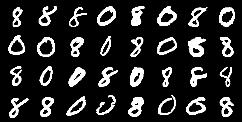
\includegraphics{images/mnist-0-8}
    \caption{Samples of digits 0 and 8 separated from the MNIST dataset.}
    \label{fig:mnist-0-8}
\end{figure}

Now it was time to test the uncertainty calculations of the predictions. First I pulled out an image of a digit 8 from the dataset and classified it (figure \ref{fig:eight}). As expected, the classifier worked well, and classified the image as being the digit 8 with a probability of 0.94. The MC dropout, with $T=1000$ (I will be using this value throughout the experiments unless otherwise mentioned), according to variation ratio was 100\% sure that the prediction has no uncertainty in it and similarly, the predictive entropy gave a value of 0.06, also indicating that the prediction has very little uncertainty for this particular sample.

\begin{figure}
    \center
    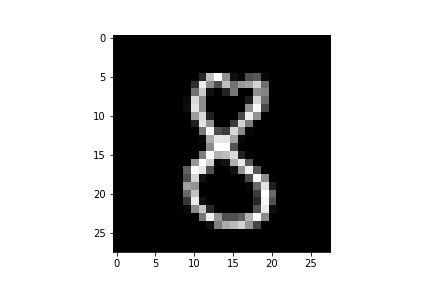
\includegraphics[scale=0.5]{images/eight}
    \caption{Sample of a digit 8 for testing predictive uncertainty.}
    \label{fig:eight}
\end{figure}

So, let's see what happens when we feed random normal noise (figure \ref{fig:gaussian-noise}) to the model. As expected, this confuses the model which predicts the random noise to be the digit 8 with a probabillity of 0.65. Now let's see what the MC dropout uncertainty estimates tell us. The variation ratio is 0.18, indicating that there is some uncertainty in the prediction. The predictive entropy is 0.41, indicating that the prediction contains very much uncertainty. Great, these results are as expected and we can continue.

\begin{figure}
    \center
    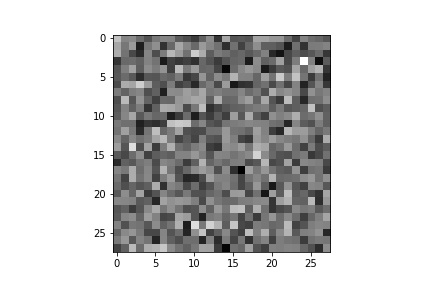
\includegraphics[scale=0.5]{images/gaussian-noise}
    \caption{Sample of standard Gaussian noise for testing predictive uncertainty.}
    \label{fig:gaussian-noise}
\end{figure}

Next I pulled out an out of distribution sample from MNIST, an image of the digit 2 (figure \ref{fig:two}) and repeated the test. This time the model gave a probability of 0.68 of the sample being of the digit 8, so it would be classified as being the digit 8. The variation ratio gave a value of 0.09, still being quite certain that the model is correct. But the predictive entropy told otherwise with a value of 0.42, meaning that the prediction has a lot of uncertainty in it. Nice, again an expected result!

\begin{figure}
    \center
    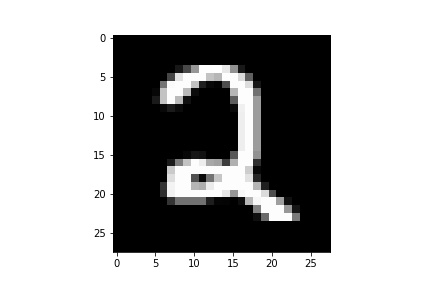
\includegraphics[scale=0.5]{images/two}
    \caption{Sample of a digit 2 for testing predictive uncertainty.}
    \label{fig:two}
\end{figure}

\subsubsection{MNIST adversarial}

I was wondering how to further test this, and got an idea: create an adversarial image of the digit 8 that the model predicts being the digit 0. By common sense, the uncertainty estimate should be high for an adversarial image. So I did just that. The resulting image can be seen in figure \ref{fig:zero-adversarial}. The model output the image being the digit 0 quite confidently, with a probability of 0.73. But the MC dropout estimates tell a different story. Again the variation ratio was not very good estimator, giving a value of 0.13, still being quite confindent that the model was correct. Instead, predictive entropy gave an uncertainty estimate of 0.47: the prediction had very much uncertainty in it. Once again a great result: we can use MC dropout to detect adversarial images! (I later found out that this has been further studied by Smith and Gal \cite{smith2018understanding}.)

Also, now it started to become obvious that the variation ratio is quite useless compared to the predictive entropy so I decided to use only precictive entropy in the future experiments. Next we'll take a look at how MC dropout works when the dataset becomes more complex.

\begin{figure}
    \center
    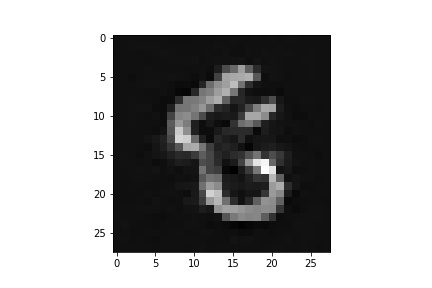
\includegraphics[scale=0.5]{images/zero-adversarial}
    \caption{An adversarial image of a digit 8 that the model predicts being digit 0 with a high probability. For human eyes this is obviously an eight, but the model predicts a zero.}
    \label{fig:zero-adversarial}
\end{figure}

\subsection{Is an ostrich a dog or a cat?}

At this point, I was quite confident that my understanding and implementation of MC dropout was correct and everything was working as expected, so it was time to move to a more challenging dataset. For simplicity I decided to stick with the binary case. A few years back I had already become familiar with the Kaggle's Dogs vs. Cats competition dataset \footnote{\url{https://www.kaggle.com/c/dogs-vs-cats-redux-kernels-edition}}, so I decided to use it for the coming experiments. Examples from the dataset can be seen in figure \ref{fig:cats-dogs}.

I decided to go for a relatively simple model that already has dropout in it. I also wanted a bit smaller model, so training would be a bit faster. The model I opted for was VGG11 (fully connected layers have dropout with a probability of 0.5), a smaller version of the quite famous VGG model \cite{simonyan15}. I froze the CNN layers, replaced the output layer to map to two outputs (dogs and cats) and then fine-tuned the classifier to classify the images. Using the one cycle policy \footnote{\url{https://pytorch.org/docs/stable/optim.html\#torch.optim.lr_scheduler.OneCycleLR}} it took just 3 epochs of training to achieve an accuracy of 0.9898 on the validation set. This was on the first try, so there was really no need to verify it on the test set.

\begin{figure}
    \center
    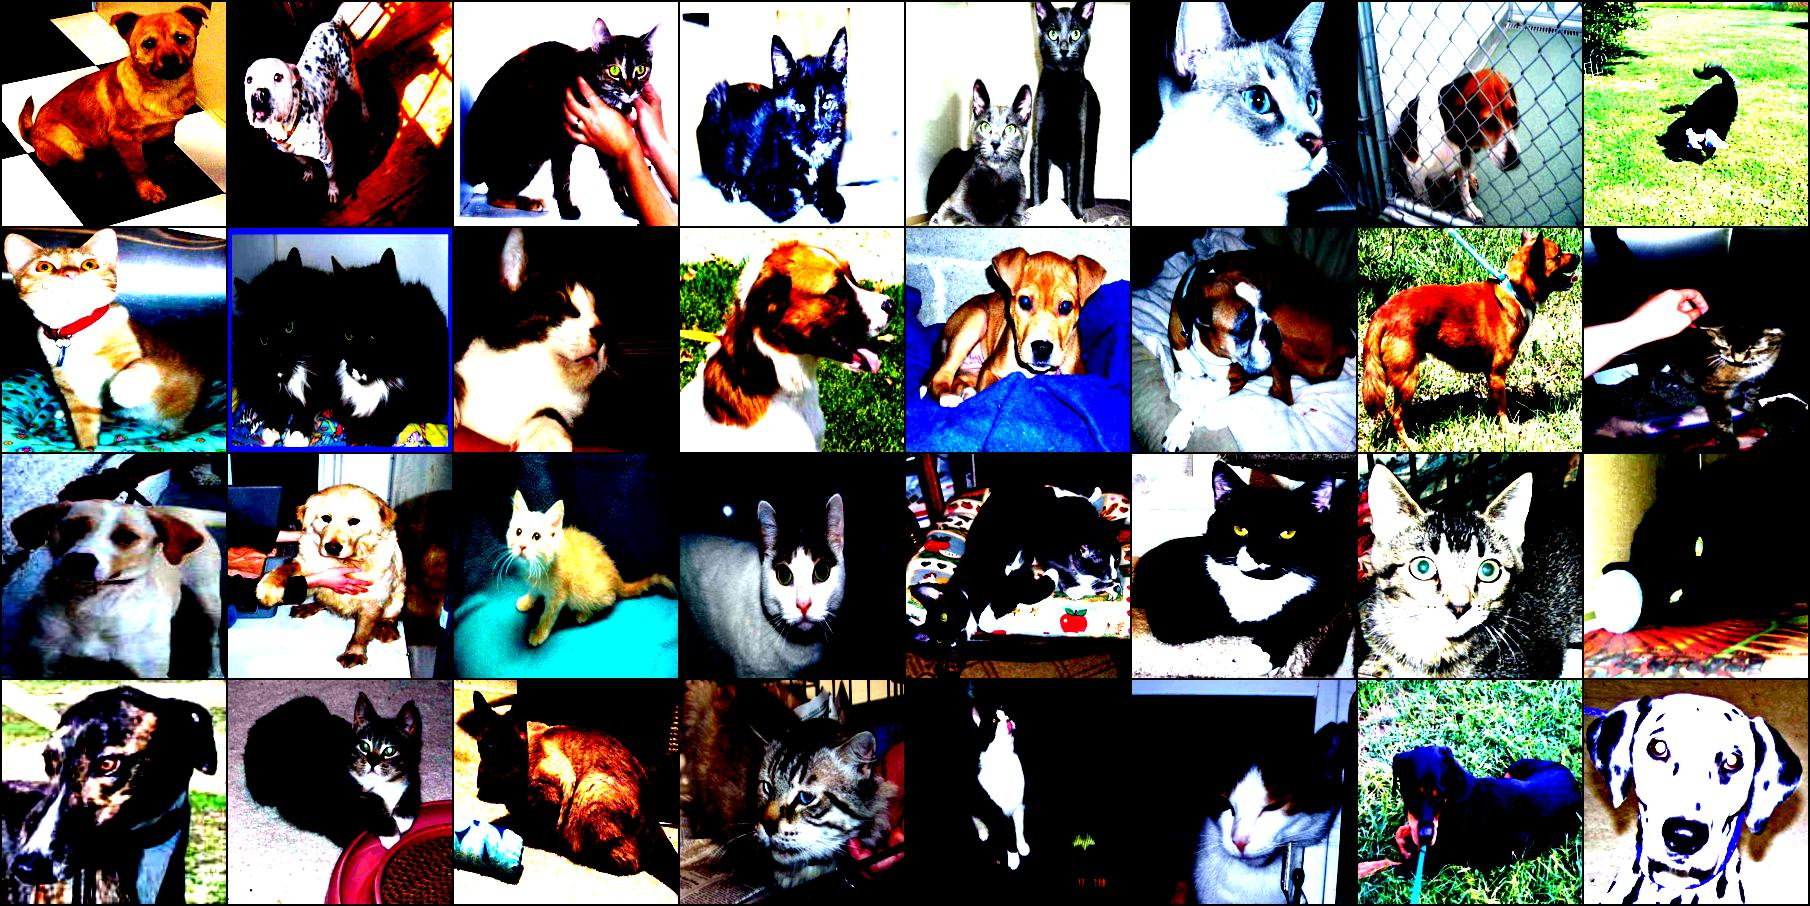
\includegraphics[scale=0.2]{images/cats-dogs}
    \caption{Training samples from the Kaggle's Dogs vs. Cats competition dataset rescaled to 224x224.}
    \label{fig:cats-dogs}
\end{figure}

Needless to say, when showing images of a cat or dog to the model the predictions were very accurate and the MC dropout predictive entropy was also telling us that the model is very certain. So, let's move on to something more exciting: an ostrich (figure \ref{fig:ostrich})!

\begin{figure}
    \center
    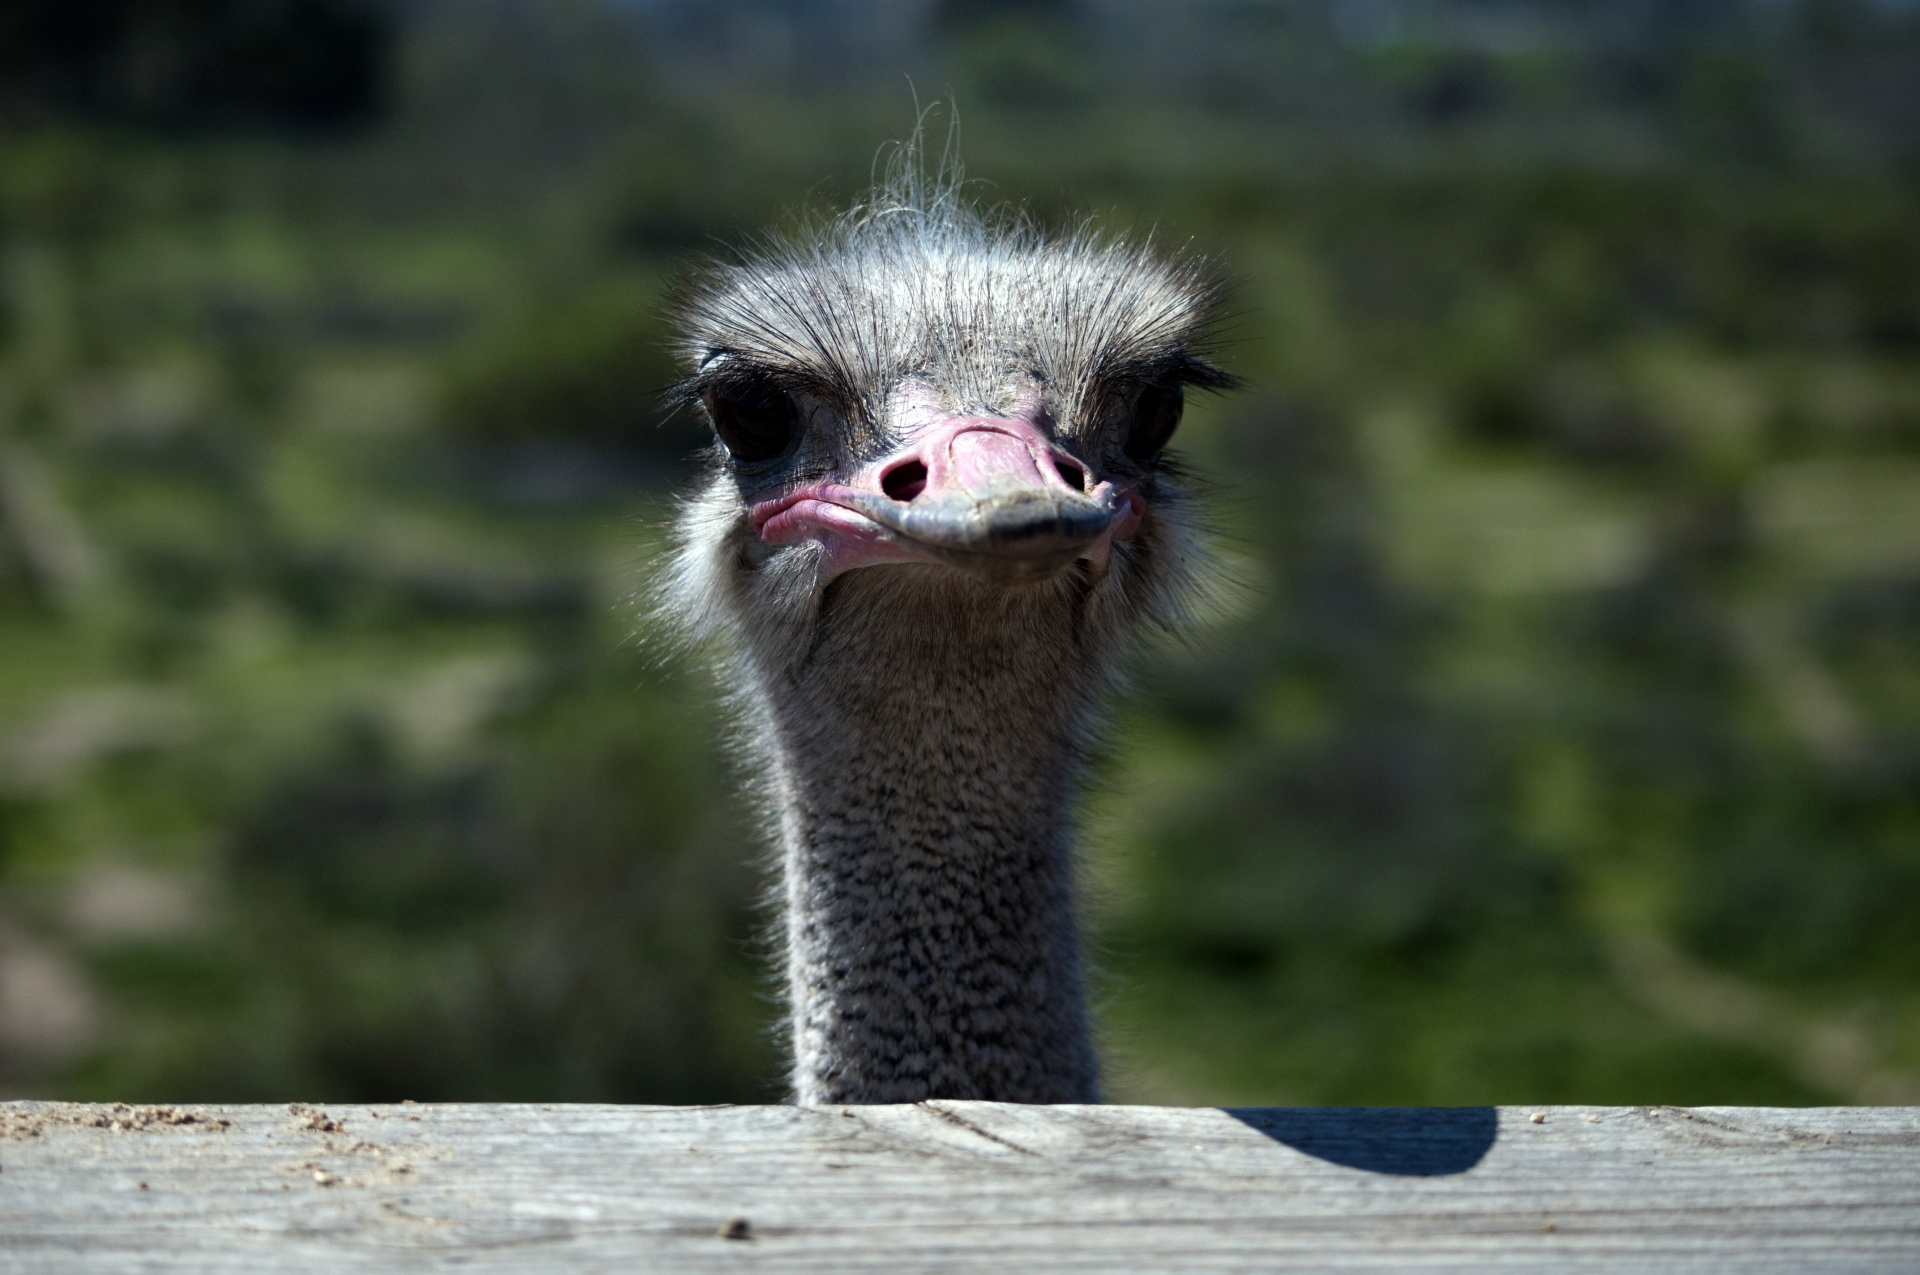
\includegraphics[scale=0.15]{images/ostrich}
    \caption{Image of an ostrich that the model, trained to classify cats and dogs, classifies as a dog with a very high probability. Image source: \url{https://www.publicdomainpictures.net/en/view-image.php?image=251857}.}
    \label{fig:ostrich}
\end{figure}

In the more complex setting the advantages of MC dropout start to kick in: our model is predicting this ostrich to actually be a dog with a whopping probability of 0.92. Now, we can check how certain the prediction is. I ran the MC dropout ($T=1000)$ algorithm and got predictive entropy of 0.36, telling us that the prediction has very much uncertainty.

According to the paper \cite{gal2016dropout}, MC dropout should work also with much smaller values of $T$, so let's see what it says about the ostrich. With $T=100$ we got a predictive entropy of 0.4. With $T=20$ the predictive entropy was 0.30. And with $T=10$ we got a predictive entropy of 0.36. So yep, even with small values of $T$ the MC dropout seems to give good results. However, it should be noted, that these are not static values but they depend on which activations the dropout happens to kill during the $T$ forward passes.

\section{Conclusions}

MC dropout seems like a very efficient and practical method to get uncertainty estimates even for existing models, given that they use dropout as regularization. However, thet method is not bulletproof: during my experiments I ran in a sample of the digit 2, that for a human observer looked like a 2, but it had very similar curves to the digit 8 and the model predicted it as the digit 8. Also the uncertainty estimates told that the prediction was very certain. Even the first ostrich I found was predicted as being a cat with very little uncertainty: probably ostriches have more similarity to cats than to dogs? (Initially I thought I had a bug and had to verify my results by testing with an image of car.) I would have wanted to include this interesting example in the report, but I wasn't sure if the image was of free license, so I decided to drop it.

Because of space and time limitations I was not able to focus on the regression part, but the basic idea is the same: make $T$ forward passes and gather $T$ models. The only difference is in how the uncertainty estimates are calculated. Also, it would have been interested to experiment with different dropout probabilities or maybe having dropout only in a single layer, but for the same reasons I did not investigate this further.

The paper \cite{gal2016dropout} is from 2016 and the field has evolved since that. There are now many more methods like MultiSWAG \cite{wilson20} and Vadam \cite{khan18} which are based on similar ideas as MC dropout, but instead of using stochasticity from dropout it is derived from weight changes; VOGN \cite{osawa19} which is based on Variational inference; and many others. The field seems to be constantly evolving, and personally I think we are going to see much more of Bayesian approaches to neural networks in the future.

\bibliographystyle{abbrv}
\bibliography{References}

\end{document}
